\documentclass[a4paper,14pt]{extarticle}

\usepackage[T2A]{fontenc}
\usepackage[utf8]{inputenc}
\usepackage[english,russian]{babel}
\usepackage[left=3cm, right=1.5cm, top=2cm, bottom=2cm]{geometry}

\usepackage{setspace}
\onehalfspacing{}

\usepackage[center]{titlesec}
\addtocontents{toc}{\protect\thispagestyle{empty}}
\usepackage[justification=centering]{caption}

\usepackage{indentfirst}
\setlength{\parindent}{20pt}

\usepackage{fancyhdr}
\setlength{\headheight}{17.0pt}
\pagestyle{fancy}
\fancyhf{}
\fancyhead[C]{\thepage}
\renewcommand{\headrulewidth}{0pt}

\usepackage[normalem]{ulem}

\hyphenpenalty=0

\usepackage[acronym]{glossaries}
\usepackage[hidelinks]{hyperref}

\usepackage{graphicx}
\graphicspath{{images/}}

\usepackage{miller}
\newcommand{\unit}[1]{ \ \text{#1}}
\newcommand{\degree}{^\circ}
\newcommand{\celcius}{^\circ \text{C}}
\newcommand{\YEu}{${(\text{Y}_{1-x}\text{Eu}_x)}_2\text{O}_3$}
\newcommand{\range}[2]{[#1\div#2]}

\usepackage{forloop}
\newcounter{x}
\newcommand{\Repeat}[2]{\forloop{x}{0}{\value{x} < #1}{#2}}
\newcommand{\writedate}{<<\Repeat{2}{\ldots}>>\Repeat{5}{\ldots}2025г.}

\usepackage{csquotes}
\bibliographystyle{gost-numeric.bbx}
\usepackage[backend=biber,
citestyle=gost-numeric,
bibstyle=gost-numeric,
sorting=none,
]{biblatex}
\addbibresource{bibliography.bib}

\usepackage{multirow}

\begin{document}
\begin{titlepage}
\thispagestyle{empty}
\begin{spacing}{1.15}
\footnotesize
\begin{center}
    МИНИСТЕРСТВО НАУКИ И ВЫСШЕГО ОБРАЗОВАНИЯ РОССИЙСКОЙ ФЕДЕРАЦИИ
    \vspace{20pt}

    ФЕДЕРАЛЬНОЕ ГОСУДАРСТВЕННОЕ АВТОНОМНОЕ ОБРАЗОВАТЕЛЬНОЕ\\
    УЧРЕЖДЕНИЕ ВЫСШЕГО ОБРАЗОВАНИЯ
    \vspace{6pt}

    «НОВОСИБИРСКИЙ НАЦИОНАЛЬНЫЙ ИССЛЕДОВАТЕЛЬСКИЙ ГОСУДАРСТВЕННЫЙ УНИВЕРСИТЕТ» (НОВОСИБИРСКИЙ ГОСУДАРСТВЕННЫЙ УНИВЕРСИТЕТ, НГУ)
    \vspace{10pt}
\end{center}
Факультет \uline{\textbf{ФИЗИЧЕСКИЙ}}
\vspace{10pt}

\noindent
Кафедра \uline{\textbf{ФИЗИЧЕСКИХ МЕТОДОВ ИССЛЕДОВАНИЯ ТВЕРДОГО ТЕЛА}}
\vspace{8mm}

\noindent
Направление подготовки \uline{\textbf{03.03.02 ФИЗИКА}}
\vspace{10pt}

\noindent
Образовательная программа: \uline{\textbf{БАКАЛАВРИАТ}}
\vspace{8mm}
\begin{center}
    \textbf{ВЫПУСКНАЯ КВАЛИФИКАЦИОННАЯ РАБОТА}

    \textbf{(научно-исследовательский формат)}
    \vspace{8mm}

    \uline{\hfill Кудрявцева Артема Леонидовича \hfill}

    $_\text{(Фамилия, Имя, Отчество автора)}$
    \vspace{8mm}
\end{center}
Тема работы \uline{Разработка прецизионного метода определения параметров элементарной ячейки для монокристального дифрактометра, оснащенного двумерным детектором \hfill}
\vfill

\noindent
\textbf{<<К защите допущена>>}

\noindent
Заведующий кафедрой \hfill \textbf{Научный руководитель}
\vspace{10pt}

\noindent
д.~ф.-м.~н., профессор \hfill д.~ф.-м.~н., профессор
\vspace{10pt}

\noindent
г.~н.~с. ИК СО РАН \hfill г.~н.~с. ИНХ СО РАН
\vspace{10pt}

\noindent
Цыбуля~С.В./\Repeat{4}{\ldots}\hfillГромилов~С.А./\Repeat{4}{\ldots}

\noindent
$_\text{(фамилия И., О.) / (подпись, МП)}$ \hfill $_\text{(фамилия И., О.) / (подпись, МП)}$
\vspace{10pt}

\noindent
\writedate\hfill\writedate{}
\vspace{8mm}

\hfill Дата защиты:\writedate{}
\vspace{8mm}

\begin{center}
    Новосибирск, 2025
\end{center}

\end{spacing}
\end{titlepage}
\tableofcontents
\section{Введение}

\subsection{Параметры элементарной ячейки}

Параметры элементарной ячейки (ПЭЯ) --- величины, определяющие метрику кристаллической решетки.
Они являются одними из основных характеристик кристаллов.
В общем случае, их представляют в виде шести различных вещественных величин: трех длин, соответствующих периодам главных направлений кристаллической решетки $(a, b, c)$, и трех углов между этими направлениями $(\alpha, \beta, \gamma)$.
Однако, благодаря симметрии кристалла, общее число независимых параметров может быть меньше: минимум одна длина $a$ в случае кубической сингонии.

На ПЭЯ кристалла влияет множество различных факторов, таких как: состав, структура, дефектность, температура, давление и другие.
Это позволяет по изменению ПЭЯ кристалла косвенно их отслеживать.
В общем случае, при значительной разнице в ПЭЯ можно говорить, что кристаллы заметно отличаются, а при достаточной точности измерений и знании того, что может отличаться --- дать количественную оценку изменения этих величин.

Однако, при небольшом их изменении, разница в ПЭЯ крайне мала.
Так, например, температурные коэффициенты расширения большинства материалов порядка $10^{-5} \unit{K}^{-1}$.
Для твердых растворов же, относительная разница значений ПЭЯ для соответствующих чистых веществ порядка $10^{-2}$, и, при изменении мольной доли на $10^{-3}$, относительное изменение ПЭЯ уже составит порядка $10^{-5}$.
Похожим образом ситуация обстоит и с остальными величинами.
Поэтому при использовании ПЭЯ для измерения косвенно связанных с ним характеристик, необходима высокая точность измерений.

Хотя, технически правильнее будет говорить не о точности, а о <<прецизионности>> измерений, от английского \textit{precision}.
В работе эти термины будут отличаться, и разница в них будет заключается в разных ошибках, которым они соответствуют.
Высокая точность будет означать, что полученные значения мало отличаются от истинного значения, а высокая прецизионность --- то, что полученные значения будут мало отличаться друг от друга.
Можно сказать, что для точных результатов систематическая ошибка значительно меньше случайной, а для прецизионности наоборот --- случайная меньше систематической.
В описанном выше случае измерения величин, слабо влияющих на ПЭЯ, систематическая ошибка практически не будет влиять на получаемые результаты, ведь обычно приходится оценивать относительную разницу величины ПЭЯ.

\subsection{Методы измерения}

Наконец, стоит рассказать о самих методах измерения ПЭЯ.
Самыми эффективными и распространенными являются различные дифракционные методы: рентгеновские, нейтронные и электронные.
Среди них самым доступным и неприхотливым является именно рентгеновская дифракция, и только она будет рассматриваться в дальнейшем.
В любой дифракции, тем не менее, основным уравнением, позволяющим, зная длину волны $\lambda$ излучения и угол дифракции $2\theta$, получить межплоскостные расстояния в кристалле $d$ является уравнение Вульфа-Брэгга~(\ref{eq:bragg}).
\begin{equation} \label{eq:bragg} 
    2 d \sin{\theta} = \lambda
\end{equation}

Установками, на которых она реализуется являются обычно лабораторные дифрактометры и специализированные станции синхротронного излучения (СИ).
Между ними, конечно, есть принципиальная разница в источнике излучения, но общая схема установки у них одинаковая.
Они состоят из:
\begin{itemize}
    \item Источника излучения
    \item Исследуемого образца
    \item Детектора излучения
\end{itemize}
В добавок к этому, каждый из этих компонентов может быть механизирован, то есть для них может регулироваться положение и ориентация в пространстве.
В качестве примера, лабораторные монокристальные дифрактометры обычно оснащаются гониометром, с помощью которого возможно точное вращение кристалла.
Так же может быть и механизирован и детектор: может регулироваться расстояние между ним и образцом, а также сам детектор обычно может вращаться вокруг образца.
Перемещение же источника возможно только для рентгеновских трубок, и это обычно реализуется в порошковых дифрактометрах.

Рентгеновские дифракционные методы отличаются между собой, и один из способов их классификации --- по виду образца: монокристальные, поликристальные, порошковые, тонкопленочные и другие.
Стандартным способом точного и воспроизводимого измерения ПЭЯ сейчас является порошковая дифракция, тогда как монокристальная используется в основном для проведения рентгеноструктурного анализа.
Может показаться странным, но данные о ПЭЯ, получаемые сейчас из рентгеноструктурного анализа по монокристальной дифракции часто являются менее достоверными и воспроизводимыми, чем порошковые данные~\cite{Dudka:2017}.
Это связано, в основном, с использованием двумерных детекторов вместо точечных.

% \subsection{Двумерные детекторы}

% Двумерные или, по-другому, матричные детекторы используют полупроводники для регистрации рентгеновских квантов.
% Есть три основных типа таких детекторов: CCD, CMOS и HPAD~\cite{Alle:2016}.

% CCD, или \textit{charge-coupled device} --- это прямые аналоги матриц, используемых для съемки в видимом диапазоне.
% Рентгеновские кванты попадая на сцинтиллятор детектора преобразуются в фотоны, которые затем преобразуются фотодиодом в электроны и собираются в потенциальные ямы, называемые пикселями детектора.
% Затем этот заряд автоматически измеряется электроникой и получается двумерное изображение, на котором интенсивность каждого пикселя напрямую связана с зарядом, накопленном в яме.

% CMOS, или \textit{complementary metal-oxide-semiconductor} --- это по-сути усовершенствованная версия CCD-матрицы.
% Главное отличие их в том, что в CMOS рядом с каждым пикселем детектора располагается небольшая электронная схема, обрабатывающая получаемый сигнал, усиливая его и нормализуя.
% Это делает данные более достоверными, уменьшая ошибки, но увеличивает размеры пикселя, а также уменьшает активную площадь потенциальной ямы для электроном, что в свою очередь уменьшая общую чувствительность детектора.

% HPAD, или \textit{hybrid pixel array detector} принципиально отличается от предыдущих двух.
% Они основываются на технологии регистрации высокоэнергетических фотонов в физике высоких энергий.
% По-сути это матрица из полупроводниковых счетчиков рентгеновских фотонов.
% В каждом таком счетчике каждый фотон напрямую в полупроводнике преобразуется в электрон-дырочные пары без промежуточного преобразования в фотоны видимого диапазона.
% Такие детекторы точнее, быстрее и эффективнее тех, что использую сцинтилляторы.

\subsection{Мотивация разработки методики}

Теперь учитывая то, что технологии детектирования рентгеновского излучения стремительно развились по сравнению с точечными детекторами, а точность определения ПЭЯ оставляет желать лучшего, то значит, что проблема монокристальной дифракции может заключаться в плохой технике эксперимента или обработке данных.
Матричные детекторы позволяют значительно увеличить объемы собираемых данных, и за короткое время можно <<просканировать>> все обратное пространство кристалла.
Но в то же время качество снимаемых рефлексов при этом неумолимо страдает.
После съемки полученные пики как-то обрабатываются программами, работающими как <<черный ящик>>, и они же выдают значения ПЭЯ.
В процессе, могут уточняться инструментальные параметры прибора, и весь набор координат пиков по-сути аппроксимируется с помощью метода наименьших квадратов (МНК).
Такой подход и дает низкую точность определения ПЭЯ при монокристальной дифракции и использовании двумерных детекторов.

Для точного определения межатомных расстояний после расшифровки структуры кристалла, важны не только относительные координаты атомов в ячейке $(x, y, z)$, но и ПЭЯ, причем с относительной точностью не хуже чем относительные координаты атомов.
Поэтому метод, который бы позволил без больших затрат точно определять ПЭЯ на первом этапе рентгеноструктурного анализа (РСтА) с тем же образцом и на той же установке позволил бы улучшить его результаты.

Также точный метод определения ПЭЯ можно использовать и для калибровки других дифракционных установок.
Хорошо измерив ПЭЯ на одном приборе, можно использовать тот же кристалл на другом приборе для его калибровки.
Впоследствии это позволит более объективно сравнивать результаты, получаемые на двух разных установках.

Все написанное выше является является мотивацией к теме работы --- разработке прецизионного метода определения ПЭЯ для малых монокристаллов на установках, оснащенных матричным детектором.
Малость монокристалла возникает из-за требования схожести образца с тем, что используется в РСтА.
% chktex-file 44
\section{Экспериментальная часть}
\subsection{Описание установки}
Рентгенографические эксперименты проводились на монокристальном дифрактометре Bruker D8 Venture (см. рисунок~\ref{fig:D8_photo}).
Его оборудование и характеристики:
\begin{itemize}
    \item Микрофокусная трубка Incoatec $I \mu S \ 3.0$
    \begin{itemize}
        \item $\text{Cu} K\alpha$ и $\text{Mo} K\alpha$ излучение
        \item Монохроматизация и коллимация с помощью многослойных зеркал Монтеля
        \item Диаметр пучка $110\unit{мкм}$
        \item Расходимость $0.3\degree$
    \end{itemize}
    \item Двумерный детектором PHOTON III
    \begin{itemize}
        \item CMOS-технология матрицы
        \item Разрешение $768 \times 1024$ пикселей
        \item Размер пикселя $135 \times 135\unit{мкм}^2$
        \item Ручная установка расстояния до образца
    \end{itemize}
    \item Трехкружный гониометр FIXED-CHI
    \begin{itemize}
        \item Гониометр использует эйлерову геометрию
        \item Автоматическая регулировка углов $\varphi$ и $\omega$ для образца и $2\theta_D$ для детектора
        \item Угол $\chi$ фиксирован и равен $54.7112\degree$
        \item Воспроизводимость установки углов $0.0001\degree$
        \item Точность установки углов $0.005\degree$\footnote{Паспортная точность установки углов не указана, но согласно результатам измерения эталонного образца на порошковом дифрактометре Bruker D8 Advance, оснащенном аналогичным гониометром, она не хуже $0.005\degree$.}
    \end{itemize}
    \item Температурная приставка Oxford Cryostream 800Plus
    \begin{itemize}
            \item Стабильность поддержания температуры $0.2\unit{К}$
    \end{itemize}
    \item Управление прибором средствами программного пакета APEX3~\cite{Bruker:2019}
\end{itemize}

Необходимо отметить, что из-за расположения рентгеновских трубок, область доступных углов для детектора оказывается ограниченной и зависящей от расстояния $D$ между образцом и детектором.

Значения характеристических длин волн, использованных в этой работе приведены в таблице~\ref{tab:wavelengths}.

\begin{table}[h]
    \centering
    \begin{tabular}{|c|c|c|}
        \hline
        Анод & $\lambda K\alpha_1,\unit{\AA}$ & $\lambda K\alpha_2,\unit{\AA}$ \\
        \hline
        Cu~\cite{Holzer:1997} & 1.54059290 (50) & 1.54442740 (50) \\
        Mo~\cite{Deslattes:1985} & 0.70931715 (41) & 0.713607 (12) \\
        \hline
    \end{tabular}
    \caption{Используемые значения длин волн}%
    \label{tab:wavelengths}
\end{table}

\begin{figure}[h]
    \centering
    \includegraphics[width=0.8\textwidth]{d8_3.jpeg}
    \caption{Фотография установки}%
    \label{fig:D8_photo}
\end{figure}

\subsection{Исследуемые образцы}
Для определения точности методики были использованы эталонные монокристаллы Si и Ge.

Монокристалл Si имел линейные размеры примерно $50 \unit{мкм}$.
Он является осколком кристалла, который ранее был исследован по методу Бонда~\cite{Lisoivan:1982}.
Значение $a = 5.430933(12)\unit{\AA}$ там было получено с использованием значение длины волны $\lambda \text{Cu} K \alpha_1 = 1.540562\unit{\AA}$.
При пересчете на более точное значение из таблицы~\ref{tab:wavelengths}, эталонное значение ПЭЯ для Si
\[ a_\text{Si} = 5.431042 (12)\unit{\AA}. \]

Монокристалл Ge также был размером около $50 \unit{мкм}$.
Его ПЭЯ измеряли в множестве работ методами Бонда, многократных отражений и многолучевой дифракции.
Полученные при этом значения ПЭЯ~\cite{Lisoivan:1982} лежат в интервале от $5.65776 (2) \unit{\AA}$ до $5.657837 (15) \unit{\AA}$.
Из них было выбрано значение $a = 5.657772 (10) \unit{\AA}$~\cite{Cooper:1962}, так как оно оказывается наиболее близким к среднему.
Пересчет для приведенного в таблице \ref{tab:wavelengths} значения длины волны дает
\[ a_\text{Ge} = 5.657885 (10)\unit{\AA} \]

Также, с целью определения однородности продукта синтеза и значения мольной доли $x$ был изучен продукт синтеза твердого раствора оксида иттрия-европия \YEu.
Для этого было отобрано 5 различных монокристаллов, ля каждого из которых был проведен РСтА и измерение ПЭЯ по разработанной методике.

\subsection{Описание методики}

Первое описание методики дано в статье~\cite{Kudryavtsev:2024:YEu}.
Общая схема проведения измерений выглядит примерно так:
\begin{enumerate}
    \item Отбор монокристалла
    \item Предварительная съемка
    \item Выбор рефлекса
    \item Съемка рефлекса
    \item Обработка профилей
    \item Расчет межплоскостного расстояния
\end{enumerate}
\subsubsection{Отбор монокристалла}
Отбор монокристалла проводится так же, как и для РСтА.
Монокристалл выбирается так, чтобы не превосходить размера первичного пучка.
В нашем случае оптимальный размер равен приблизительно 50~мкм.
\subsubsection{Предварительная съемка}
Предварительная съемка проводится с целью определения ориентации кристалла, его дифракционного класса и получения данных об интенсивности рефлексов.

Сама съемка состоит серии полных сканирований при вращении вокруг оси $\varphi$ с шагом $0.5\degree$ для при фиксированном угле $\omega$.
Три таких сканирования выполняются при углах детектора $2\theta_D = \{-45\degree, 0\degree, 45\degree\}$ при фиксированном расстоянии до образца $D \approx 70\unit{мм}$.

Обработка снимков и получение ориентации производится в программе APEX3.
На выходе программы получается файл формата p4p, где информация об ориентации кристалла содержится в виде UB матрицы~\cite{Busing:1967}.

\subsubsection{Выбор рефлекса}
Выбор рефлекса для съемки происходит так, чтобы погрешность измерений была минимальной.
Основными критериями в таком случае оказываются наибольшие угол $2\theta$ и интенсивность рефлекса.
При этом необходимо учитывать геометрию установки, так как не все рефлексы оказывается возможно вывести в отражающее положение для двух симметричных положений в экваториальной плоскости.

Средствами программы APEX3 производить такой перебор рефлексов неэффективно и крайне проблематично, так как программа рассчитывает для одного рефлекса максимум только одну пару углов $(\varphi, \omega)$ из двух возможных в общем случае.
Поэтому была специально написана программа~\cite{Kudryavtsev:2024:eccentr} для перебора всех рефлексов, расчета для них углов гониометра и отбора случаев когда в оказывается возможным вывести рефлекс в два симметричных положения, а также когда доступна для выведения и его фриделевская пара.

Программа позволяет находить среди множества плоскостей, связанных симметрией такие, которые можно вывести в отражающее положение хотя бы при одном (из двух симметричных) положений детектора.
Для этого используется информация о текущей ориентации кристалла на гониометре, т.е. p4p-файл, в котором находится матрица ориентации UB и предварительные значения ПЭЯ.
Используя известную длину волны, размеры пикселя, расстояние до детектора, и другие неизменные параметры прибора, программа вычисляет углы гониометра $(\varphi, \omega)$, необходимые для выведения каждой плоскости в отражающее положение на экваториальную плоскость.
В каждом случае проверяются геометрические ограничения прибора.
Полученная информация для всех подходящих рефлексов собирается в таблицу Excel, ее можно проанализировать и провести отбор.
\subsubsection{Съемка рефлекса}
Съемка рефлекса представляет собой сканирование при вращении вокруг оси $\omega$ в диапазоне $\pm 2\degree$ относительно рассчитанного значения $\omega$ для отражающего положения.
Время съемки выставлялось таким, чтобы максимум на профиле пика составлял не менее 10000~имп.

В программе APEX3 невозможно выставить время съемки больше, чем 600~с, поэтому для достижения последнего условия производились несколько одинаковых съемок, пока не была достигнута требуемая интенсивность.
\subsubsection{Обработка профилей}
Обработка профилей состоит из нескольких этапов, по завершению которых можно рассчитать межплоскостное расстояние.
Реализована она была тоже в виде программы~\cite{Kudryavtsev:2024:eccentr}.

На входе она использует p4p-файл и информацию о примерном положении центра детектора (результат юстировки, прямое определение, калибровка).
Из экспериментального фрейма вырезается центральная область $X = \pm 30\unit{пикс.}, Y = \pm 15\unit{пикс.}$, в которой, исходя из условия $2\theta_D \approx 2\theta$, должен находиться искомый рефлекс.
Медианное значение интенсивности принимается за начальное значение фона.
Пиксели с интенсивностью больше заранее заданной принимаются за ''горячие пиксели'' и их значения приравниваются среднему значению по 8 соседним пикселям.
После учета горячих пикселей максимум интенсивности в выбранной области назначается примерным положением $K\alpha_1$--составляющей.
Далее, исходя из значений $D$ и $2\theta$ рассчитывается положение $K\alpha_1$--составляющей и обе точки смещаются так, чтобы теоретическое положение $K\alpha_1$ совпадало с координатами найденного максимума интенсивности.
Аппроксимация дублета проводится двумя независимыми  функциями 2D-Gauss, т.е. без закрепления междублетного расстояния и соотношения интенсивностей составляющих $2/1$.
Направлениями главных осей берутся вдоль координат детектора $X$ и $Y$ детектора.
В наших экспериментах именно функция 2D-Gauss наиболее хорошо описывала форму пика при минимальном числе уточняемых параметров: координаты максимума, полуширины (ширина на половине высоты, FWHM) в направлениях $X$ и $Y$, и интегральная интенсивность.

\subsubsection{Рассчет межплоскостного расстояния}
Для достаточно малой разницы координат рефлексов искомый угол дифракции можно рассчитать по формуле
\begin{equation} \label{eq:bond2}
    2\theta = 2\theta_D - \frac{\gamma}{2} (X_{+} - X_{-}),
\end{equation}
где $\gamma$ --- угловой размер пикселя в точке детектирования рефлекса, $X_{-}, X_{+}$ --- координаты рефлексов при отрицательном и положительном углах детектора.
В формуле $2\theta_D$ предполагается положительным.
Знак перед разницей координат рефлексов зависит от направления координаты $X$ детектора и направлением положительного вращения детектора вокруг оси $2\theta_D$.
Если они направлены в разные стороны, то знак ``$-$'', если в одну, то ``$+$''.
В нашей установке направления выбраны так, что перед разницей должен быть ``$-$''.
\subsection{Учет эксцентриситета}
Дополнительная съемка фриделевских пар позволяет учитывать эффект смещения кристалла при вращении вокруг оси $\omega$.
Так как рефлекс при съемке выводится в экваториальную плоскость, то угол $\omega$ для фриделевской пары изначального рефлекса отличается на $180\degree$.
Так как при повороте на $180\degree$ положение кристалла как бы отражается относительно оси $\omega$, то среднее значение координат рефлексов в этих двух положения будет соответствовать положению кристалла ровно на оси $\omega$~\ref{fig:eccentr}.

\begin{figure}[ht!]
    \centering
    
\includegraphics[width=0.8\textwidth]{eccentr.png}
    \caption{Схемы эксперимента для учета эксцентриситета образца.}\label{fig:eccentr}
\end{figure}

Таким образом измерение фриделевской пары позволяет использовать уточненное значение координат рефлекса
\[X_{true} = \frac{1}{2}(X + X_{frid})\]
где $X, X_{frid}$ --- координаты обычного рефлекса и его фриделевской пары соответственно.
Подставляя это в формулу~\ref{eq:bond2} получим
\begin{equation} \label{eq:bond4}
    2\theta = 2\theta_D - \frac{\gamma}{4} (X_{+} + X_{+frid} - X_{-} - X_{-frid}).
\end{equation}
\subsection{Расчет углового размера пикселя}
Зная линейные размеры пикселя $P$ и расстояние до центра детектора $D$ можно с хорошей точностью рассчитать угловой размер пикселя как
\begin{equation} \label{eq:gamma_simple}
    \gamma = \frac{P}{D}.
\end{equation}
В нашем случае $P = 135\unit{мкм}$, а расстояние $D$, указываемое прибором $D = 128.53\unit{мм}$.

Однако значение $D$, которое показывает прибор, всегда можно поставить под сомнение.
Правильнее провести калибровку положения детектора, например, согласно методике~\cite{Panchenko:2023}.
Для этого съемка эталонного монокристалла Si была проведена путем $\omega$--сканирования интервалов $10\degree$ в области углов $200\degree$ при пяти положениях кристалла по углу $\varphi$ (шаг $10\degree$).
Обработка полученных фреймов проведена по программе SearchXY~\cite{Panchenko:2023}.
В результате получено значение $D = 128.21\unit{мм}$.
Развороты детектора в наших экспериментах можно не учитывать из-за их малости и так как регистрация рефлексов проводится центральной областью детектора.

Полная калибровка занимает достаточно много времени и не всегда целесообразна.
Другой подход к определению $\gamma$ основан на съемке одного и того же рефлекса при двух угловых положениях детектора.
Так, рефлекс $\hkl(11 3 1)$ эталонного монокристалла Si был отснят при $2\theta_D = 96.4\degree, 97.0\degree$.
Смещение рефлекса $\Delta X$ позволяет провести вычисление $\gamma$ по формуле
\begin{equation} \label{eq:gamma_delta}
    \gamma = \frac{\Delta 2\theta_D}{\Delta X}
\end{equation}

Отметим, что такой подход позволяет проводить измерения при минимальных отклонениях рефлекса от центра детектора.
Полученное значение идеально совпадает с результатом, полученным по результатам полной калибровки.
Итоговое значение, использовавшееся далее
\[ \gamma = 0.06033\degree \]
\section{Изучение эталонных кристаллов Si и Ge}

Для измерения ПЭЯ Si, с учетом ранее обозначенных приборных ограничений, наиболее подходят три семейства кристаллографических плоскостей \hkl{11 3 1}, \hkl{9 7 1} и \hkl{9 5 5} c $2\theta = 96.737\degree$.
В случае Ge выбраны семейства \hkl{10 6 0} и \hkl{8 6 6} с $2\theta = 93.949\degree$.
Поиск подходящих рефлексов средствами программы APEX3 можно сделать только в ручном режиме, т.е. последовательно прелагая значения \hkl(h k l).
Возможны два варианта расчетов: первый предполагает определение углов для вывода кристаллографического направления навстречу пучку ($\varphi_0$ и $\omega_0$), второй --- углов для установки кристаллографической плоскости в отражающее положение при положении детектора в отрицательных углах $2\theta_D$.
В обоих вариантах предлагается только одно значение $\varphi$ (из двух возможных).
Такого функционала совершенно недостаточно для учета эксцентриситета образца: согласно~\cite{Ponomarev:1969} необходимо подобрать пару рефлексов \hkl(h k l), которые можно зафиксировать при положениях гониостата $\omega \approx \pm 90\degree$ (см. рис.~\ref{fig:eccentr}).
В случае Si, число симметрично связанных плоскостей равно 120 (для Ge –-- 48) и сделать это средствами программы APEX3 проблематично.
Необходимые расчеты были проведены по программе James.

\begin{figure}[ht!]
    \centering
    \begin{subfigure}{0.5\textwidth}
    \centering
    
\includegraphics[]{eccentr.pdf}
    \caption{}%
    \label{fig:eccentr_neg}
    \end{subfigure}%
    \begin{subfigure}{0.5\textwidth}
    \centering
    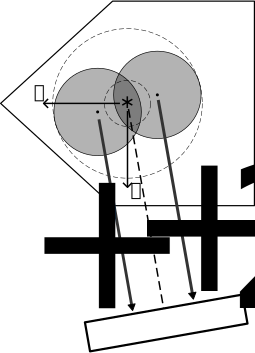
\includegraphics[]{eccentr_2.pdf}
    \caption{}%
    \label{fig:eccentr_pos}
    \end{subfigure}
    \caption{
        Схемы эксперимента для учета эксцентриситета образца, связанного с поворотом вокруг оси $\omega$ (ось $\omega$ идет перпендикулярно плоскости чертежа, выход показан звездочкой).
        a --- показаны два положения образца (условные центры обозначены жирными точками), при которых проводятся съемки рефлексов и определяются положения максимумов – $X_1$ и $X_2$.
        Окружность меньшего диаметра соответствует сфере сведения, большая окружность (выделена пунктиром) ограничивает область расположения образца.
        Показана система координат: направление $x$ проходит через ось $\omega$ в направлении первичного пучка (условно показано, что в общем случае $x$ не совпадает с максимумом первичного пучка);
        $y$ --- направление перпендикулярное $x$ и лежащее в экваториальной плоскости.
        Направление $z$ совпадает с осью $\omega$.
        b --- схема для симметричного положения детектора.
    }%
    \label{fig:eccentr}
\end{figure}

Первая часть программы James позволяет находить среди множества плоскостей, связанных симметрией такие, которые можно вывести в отражающее положение хотя бы при одном (из двух симметричных) положении детектора.
Для этого используется информация о текущей ориентации кристалла на гониометре, т.е. p4p-файл, в котором находится матрица ориентации UB~\cite{Busing:1967} и предварительные значения ПЭЯ.
Углы гониометра $\varphi$ и $\omega$, необходимые для выведения каждой плоскости в отражающее положение на экваториальную плоскость, вычисляются исходя из известной длины волны, размеров пикселя, расстояния до детектора и других неизменных параметров прибора.
В каждом случае проверяются геометрические ограничения прибора.
Полученная информация для всех подходящих рефлексов собирается в таблицу Excel, ее можно проанализировать и провести отбор.

Вторая часть программы James связана с обработкой полученных фреймов, т.е. описанием 2D-профиля дублета. На входе она использует p4p-файл и информацию о примерном положении центра детектора (результат юстировки, прямое определение, калибровка).
Из экспериментального фрейма вырезается центральная область ($X = \pm 30\unit{пикс.}$, $Y = \pm 15\unit{пикс.}$), в которой, исходя из $2\theta_D \approx 2\theta_{hkl}$, должен находиться искомый рефлекс.
Медианное значение интенсивности принимается за начальное значение фона.
Пиксели с интенсивностью больше заранее заданной принимаются за ''горячие пиксели'' и их значения приравниваются среднему значению по 8 соседним пикселям.
После учета горячих пикселей максимум интенсивности в выбранной области назначается примерным положением $K\alpha_1$-составляющей.
Далее, исходя из значений $D$ и $2\theta$ рассчитывается положение $K\alpha_2$-составляющей и обе точки смещаются так, чтобы теоретическое положение $K\alpha_1$ совпадало с координатами найденного максимума интенсивности.
Аппроксимация дублета проводится двумя независимыми  функциями 2D-Gauss, т.е. без закрепления междублетного расстояния и соотношения интенсивностей составляющих $2/1$.
Направлениями главных осей берутся вдоль координат детектора $X$ и $Y$ детектора.
В наших экспериментах именно функция 2D-Gauss наиболее хорошо описывала форму пика при минимальном числе уточняемых параметров: координаты максимума, полуширины (ширина на половине высоты, FWHM) в направлениях $X$ и $Y$, и интегральная интенсивность.

\subsection{Оценка и учет эксцентриситета образца Si}

Несмотря на тщательную центрировку образца (в том числе с контрольными разворотами по оси $\omega$) крайне сложно точно определить центр образца, особенно при его неопределенной форме.
Можно ожидать, что при повороте вокруг оси $\omega$ центр образца движется по окружности, а сам образец описывает торообразную поверхность, ее условный внешний контур показан на рис.~\ref{fig:eccentr} штриховой окружностью.
Выход оси $\omega$ показан звездочкой: считаем, что в общем случае ось не пересекается центром первичного пучка.
Подобную картину можно ожидать и при повороте образца вокруг оси $\varphi$.
Так как для использованного гониометра паспортное значение диаметра сферы сведения осей (sphere of confusion) составляет 7~мкм, центр образца при повороте вокруг обеих осей движется по достаточно сложной траектории.

Для оценки смещений центра образца при повороте вокруг оси $\varphi$, среди доступных для измерения рефлексов от семейств кристаллографических плоскостей типа \hkl{11 3 1}, \hkl{9 7 1} и \hkl{9 5 5}, было выбрано 10 вариантов, у которых значения $\omega$ лежат в интервале от $-82\degree$ до $-95\degree$.
Это примерно соответствует позиции образца при центрировании.
Все съемки проведены при положении детектора: $2\theta_D = -96.7\degree$, $D = 128.53\unit{мм}$.
Зависимость $X(\varphi)$ представлена на рис.~\ref{fig:eccentrSi}а.
Интервал значений $X$ составляет $\approx 0.3$~пикселя, что с учетом размера пикселя, соответствует смещениям центра образца с оси $\varphi$ на 20~мкм.

\begin{figure}[ht!]
    \centering
    \includegraphics[width=0.8\textwidth]{eccentrSi.png}
    \caption{
        Смещение максимумов дифракционных отражений Si \hkl(11 3 1), \hkl(9 7 1) и \hkl(9 5 5) по оси $X$ детектора из-за эксцентриситета образца: a --- зависимость координаты $X$ от угла $\varphi$ (значения углов $\omega \approx 270\degree$);
        b --- зависимость координаты $X$ от угла $\omega$ (значения углов $\varphi$ лежат в интервале $\range{283.6}{300.7}\degree$)
    }%
    \label{fig:eccentrSi}
\end{figure}

Таким образом, два проведенных эксперимента показали одинаковые картины эксцентриситетов, связанных с поворотами образца вокруг осей $\omega$ и $\varphi$.
При измерении ПЭЯ наиболее разумно исключить влияние именно последнего, тогда далее можно использовать подход, предложенный в~\cite{Ponomarev:1969}.
Он заключается в съемке фриделевской пары со значениями $\omega \approx \pm 90\degree$, что соответствует крайним положениям центра образца в направлении первичного пучка.
На рис.~\ref{fig:eccentr} центры образцов показаны жирными точками.
Очевидно, что при таких положениях образца можно ожидать максимальных смещений дифракционных рефлексов.
Среди всех вариантов, предложенных программой James, были выделены 5 фриделевских пар, удовлетворяющих этому критерию.
Их индексы и установочные углы $\varphi$ и $\omega$ представлены в табл.~\ref{tab:Si} Приложения.
Там же даны координаты максимумов рефлексов, зарегистрированных при симметричных положениях детектора $2\theta_D = 96.7\degree$ и средние значения для каждой пары $\left<X\right> = (X_1 + X_2) / 2$.
Как следует из рис.~\ref{fig:eccentr} значения $\left<X\right>$ соответствует мнимому положению кристалла на оси вращения $\omega$.
Для учета эксцентриситета в формуле~(\ref{eq:bond2}) вместо значений $X$ необходимо использовать значения $\left<X\right>$.
Чтобы различать рефлексы, зарегистрированные при симметричных положениях детектора, введем надстрочные индексы <<$-$>> и <<$+$>>, тогда выражение~\ref{eq:bond2} можно представить в следующем виде:
\begin{equation}\label{eq:bond4}
    2\theta_{hkl} = 2\theta_D + \gamma (\tensor*[^-]{X}{_1} + \tensor*[^-]{X}{_2} - \tensor*[^+]{X}{_1} - \tensor*[^+]{X}{_2}) / 4 = 2\theta_D + \gamma (\left<\tensor*[^-]{X}{}\right> - \left<\tensor*[^+]{X}{}\right>) / 2
\end{equation}
где $\gamma$ --- угловой размер пикселя.

\subsection{Определение угловых размеров пикселя}

При регистрации рефлекса центральной областью детектора (как в нашем случае) значение $\gamma$ можно вычислить исходя из физических размеров пикселя $P$ (в нашем случае 0.1353~мм) и расстояния от образца до детектора $D$ (в нашем случае 128.53~мм) по формуле:
\begin{equation}\label{eq:pixsize}
    \gamma = \frac{P}{D}
\end{equation}
Однако значение $D$, которое показывает прибор, всегда можно поставить под сомнение.
Правильнее провести калибровку положения детектора, например, согласно методике~\cite{Panchenko:2023}.
Для этого съемка эталонного монокристалла Si была проведена путем $\omega$-сканирования интервалов $10\degree$ в области углов $200\degree$ при пяти положениях кристалла по углу $\varphi$ (шаг $10\degree$).
Обработка полученных фреймов проведена по программе SearchXY~\cite{Panchenko:2023}.
В результате получено значение $D = 128.21\unit{мм}$.
Развороты детектора (rot1, rot2, rot3) в наших экспериментах можно не учитывать, т.к. регистрация рефлексов проводится центральной областью детектора.
Итоговое значение $\gamma = 0.06033\degree$.

Не всегда проведение полной калибровки положения детектора целесообразно, т.к. она занимает достаточно много времени.
Можно согласно~\cite{Gromilov:2022} использовать данные о положении $K\alpha_1$- и $K\alpha_2$-составляющих любого из изученных рефлексов эталона, тогда по разнице значений $X$ и теоретическим положениям углов $2\theta$  $K\alpha_{1,2}$-составляющих значение $\gamma$ вычисляют по формуле:
\begin{equation}\label{eq:pixsize_exp}
    \gamma = \frac{2\theta_2 - 2\theta_1}{\Delta X}
\end{equation}

Другой подход к определению $\gamma$ основан на съемке одного и того же рефлекса при двух угловых положениях детектора.
Так, рефлекс \hkl(-11 1 -3) Si был отснят при $2\theta_A = 96.4\degree$ и $2\theta_B = 97.0\degree$.
Смещение максимума $\Delta X$ позволяет провести вычисление $\gamma$ по формуле:
\begin{equation}\label{eq:pixsize_exp_2}
    \gamma = \frac{2\theta_A - 2\theta_B}{\Delta X} = 0.06033\degree
\end{equation}

Отметим, что такой подход позволяет проводить измерения при минимальных отклонениях рефлекса от центра детектора.
Полученное значение идеально совпадает с результатом, полученным по результатам полной калибровки.

\subsection{Вычисление ПЭЯ Si}

Полученное значение $\gamma$ позволяет вычислить $a_\text{Si}$.
При произвольном выборе рефлексов из табл.~\ref{tab:Si} Приложения расчет согласно~\ref{eq:bond2} приводит к значениям угла $2\theta$ в интервале $\range{96.722}{96.747}\degree$: отклонения от теоретического значения $96.734\degree$ достигают $0.013\degree$.
Учет эксцентриситета согласно~\ref{eq:bond4} с использованием произвольных пар средних значений $\left<\tensor*[^-]{X}{}\right>$ и $\left<\tensor*[^+]{X}{}\right>$ уменьшает интервал значений $2\theta$ до $\range{96.730}{96.736}\degree$ а отклонения от теоретического значения не превышают $0.004\degree$.
Использование рефлексов с близкими значениями углов $\varphi = -66.31\degree$ и $59.35\degree$ (индексы рефлексов выделены в табл.~\ref{tab:Si} Приложения жирным) позволяет учесть эксцентриситет, связанный с поворотом образца вокруг оси $\varphi$.
Конечные результаты уточнения: $2\theta = 96.732\degree$, $d = 0.47452 (3)\unit{\AA}$, $\Delta d / d = 6.2 \cdot 10^{-5}$, $a = 5.4311(3)\unit{\AA}$ (в скобках указаны абсолютные погрешности, вычисленные для $\Delta 2 \theta = 0.004\degree$).
Можно отметить, что полученное значение $a_\text{Si}$ отклоняется от эталонного всего на $0.00006\unit{\AA}$.
Чтобы полностью исключить влияние эксцентриситета, связанного с поворотом кристалла вокруг оси $\varphi$, необходимо вывести одно из кристаллографических направлений вдоль оси $\omega$, тогда измерения можно проводить на рефлексах типа \hkl{h k 0}.
При использовании гониометра с изменяемым углом $\chi$ (т.е. четырехкружного) такая проблема не возникает.
В нашем случае угол $\chi$ на гониометре фиксирован, а штатные гониометрические головки предполагают только линейные перемещения образца.

\subsection{Вычисление ПЭЯ Ge}

Для устранения эксцентриситета, связанного с поворотом кристалла вокруг оси $\varphi$ монокристалл Ge был смонтирован на оригинальной гониометрической головке, имеющей возможность поворота образца вокруг одной оси на $\pm 10\degree$ (далее гониометрическая $\chi$-головка).
После определения ориентации кристалла, с помощью программы James были рассчитаны углы для выведения кристаллографического направления вдоль оси $\omega$, для этого был использован следующий алгоритм.

Повороты образца описываются эйлеровыми углами $\varphi$, $\omega$ и $\chi$.
Правосторонняя декартова система координат гониометра задана следующим образом.
Направление оси $x$ совпадает с направлением первичного пучка.
Если смотреть навстречу $x$, то положительным изменением угла $\omega$ будет вращение против часовой стрелки.
Ось $z$ выбирается в направлении оси $\omega$ и против направления оси $\varphi$ (в нулевом положении для четырехкружного гониометра).
Направление оси $y$ задается автоматически.
Ось $\chi$ направлена против оси $x$, в нашем случае соответствующий ей угол поворота фиксирован и равен приблизительно $55\degree$.

Нулевой угол дуги нашей гониометрической головки обозначим $\chi^\ast$.
Т.к. кристаллографическое направление можно вывести вдоль или против $z$, то число возможных вариантов $\chi$ и $\chi^\ast$ может быть равно 4 (2 в вырожденном случае) или 0 (если процедура невозможна).
Ограничение значений угла $\chi^\ast$ связано с диапазоном углов дуги гониометрической головки, в нашем случае $\pm 10\degree$.

Если задать кристаллографическое направление \hkl[h k l] в виде трехмерного вектора $s$, получающегося домножением вектора-столбца \hkl(h k l) на матрицу ориентации UB, то определить возможность выведения рефлекса можно по углу $\theta_s$ между $s$ и $x$ и полярному углу $\varphi$ проекции $s$ на плоскость $yz$ (рис.~\ref{fig:scheme}).
Кристаллографическое направление можно вывести вдоль оси $\omega$ если $\sin{\theta_s} > \cos{\chi}$.
В этом случае углы $\chi^\ast$ будут равны:
\[ \varphi_s - \arcsin\left(\frac{\cos{\chi}}{\sin{\theta_s}}\right) \]
\[ \varphi_s + \arcsin\left(\frac{\cos{\chi}}{\sin{\theta_s}}\right) + 180\degree \]
\[ \varphi_s + \arcsin\left(\frac{\cos{\chi}}{\sin{\theta_s}}\right) \]
\[ \varphi_s - \arcsin\left(\frac{\cos{\chi}}{\sin{\theta_s}}\right) + 180\degree \]

При значении $\cos{\chi} > 0$ первые два угла соответствуют выведению $s$ вдоль $x$, а другие --- $-x$. При смене знака $\cos{\chi}$ картина меняется на противоположную.
Соответствующие углы $\omega$ будут равны:
\[\arctan\left(-\sqrt{\sin^2{\theta_s} - \cos^2{\chi}}, -\cos{\theta_s}\right)\]
\[\arctan\left(\sqrt{\sin^2{\theta_s} - \cos^2{\chi}}, -\cos{\theta_s}\right)\]
\[\arctan\left(\sqrt{\sin^2{\theta_s} - \cos^2{\chi}}, \cos{\theta_s}\right)\]
\[\arctan\left(-\sqrt{\sin^2{\theta_s} - \cos^2{\chi}}, \cos{\theta_s}\right)\]

где $\arctan(y, x)$ –-- полярный угол точки с координатами $(x, y)$ на координатной плоскости. 

\begin{figure}[ht!]
    \centering
    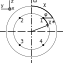
\includegraphics{scheme.pdf}
    \caption{
        Схема направления осей гониометра ($\varphi$, $\chi$, $\omega$) и дополнительного поворота монокристалла на гониометрической головке ($\chi^\ast$) в проекции $yz$.
        Экваториальная плоскость гониометра показана пунктирной линией.
        Вектор кристаллографического направления $s$ показан стрелкой.
        Путь поворота вектора по трем углам $\chi^\ast$, $\varphi$, $\chi$ обозначен жирной ломаной линией.
        Точки 1--4 обозначают 4 возможные положения, через которые кристаллографическое направление может быть выведено вдоль или навстречу оси $\omega$.
    }%
    \label{fig:scheme}
\end{figure}

Расчеты для монокристалла Ge показали, что вдоль оси $\omega$ можно вывести направление \hkl{0 1 0}, т.к. для него значение угла $\chi^\ast = 2.2\degree$.
После соответствующего поворота образца на гониометрической $\chi$-головке, исследование в схеме Бонда было проведено по рефлексам типа \hkl{10 0 6} (теоретическое значение $2\theta = 93.943\degree$).
Все рефлексы регистрировали при одинаковых значениях угла $\varphi = -179.06\degree$.
Приборные ограничения позволили отснять только 12 из 16 теоретически возможных рефлексов, координаты их максимумов приведены в табл.~\ref{tab:Ge} Приложения.
При произвольных сочетаниях рефлексов, возможны 36 вариантов пар, тогда значения $2\theta$, вычисленные согласно~\ref{eq:bond2}, лежат в интервале $\range{93.935}{93.958}\degree$.
Максимальные отклонения от теоретического значения достигают $0.015\degree$.
Для учета эксцентриситета согласно~\ref{eq:bond4} были использованы 4 пары значений $\left<X\right>$, при этом вычисленные значения $2\theta$ укладываются в узкий интервал $\range{93.943}{93.945}\degree$, а отклонения от теоретического значения не превышают $0.001\degree$.
Если использовать среднее значение $2\theta = 93.945\degree$, то: $d = 0.48515 (3)\unit{\AA}$, $\Delta d / d = 6.5 \cdot 10^{-5}$, $a = 5.6578 (4)\unit{\AA}$.
Отклонение полученного $a_\text{Ge}$ от теоретического значения $5.657885\unit{\AA}$ составляет 
$0.0001\unit{\AA}$.

Анализ координат $Y$ рефлексов Ge (см. табл.~\ref{tab:Ge} Приложения) позволяет оценить точность выведения направления $b$ вдоль оси $\omega$.
Для этого можно построить зависимости $Y$ от $\omega$ для экспериментов, проведенных при двух симметричных положениях детектора $2\theta_D = 93.9\degree$.
В обоих случаях зависимости хорошо описываются синусоидами, но при $2\theta_D = -93.9\degree$ фаза сдвигается на $\theta$, а при $2\theta_D = +93.9\degree$ на $\theta + 180\degree$.
Для одновременной обработки всех рефлексов значения сдвигов вычитали из первичных значений $\omega$.
Из построенной аппроксимации (см. рис.~\ref{fig:eccentrGe}) следует, что максимальная разница значений $Y$ составляет $\approx 2.2\unit{пикс.}$, что соответствует отклонению направления $b$ от оси $\omega$ $0.13\degree$.
Такой показатель соответствует цене нониусной шкале дуги использованной гониометрической головки.
Т.к. отклонение лежит в плоскости дуги гониометрической головки, можно утверждать, что оно связано преимущественно именно с погрешностью установки угла $\chi^\ast$, а не угла $\varphi$.

\begin{figure}[ht!]
    \centering
    \includegraphics[height=0.5\textwidth]{eccentrGe.png}
    \caption{
        Зависимость координат $Y$ от угла $\omega$ для монокристалла Ge.
        Точки полученные при положении детектора $2\theta_D = -93.9\degree$ обозначены кружками, а при $2\theta_D = +93.9\degree$ --- квадратами.
        Аппроксимация всех точек проведена с помощью МНК, использована функция $Y = a_0 + a_1 \cos(\omega - \omega_1)$
    }%
    \label{fig:eccentrGe}
\end{figure}

Выведение кристаллографического направления вдоль оси $\omega$ позволяет не только определять межплоскостные расстояния и ПЭЯ, но и углы между кристаллографическими плоскостями типа \hkl[h 0 l].
Так, для изученного монокристалла Ge было проведено измерение угла между плоскостями \hkl[6 0 -10] и \hkl[10 0 -6].
Для этого получена зависимость интенсивности рефлекса от угла $\omega$ с помощью $\omega$-сканирования диапазона $0.4\degree$, содержащего максимум интенсивности рефлекса от $K\alpha_1$ с шагом $0.002\degree$.
Для каждой позиции проводили суммирование интенсивности всех пикселей в прямоугольной области детектора $50\times30$.
Значение угла $\omega$, при котором достигается максимальная интенсивность, было получено аппроксимацией полученной зависимости $I(\omega)$ полиномом второй степени.
В результате, полученные значения углов $\omega$ составили $67.6113 (2)\degree$ и $95.6731 (2)\degree$ для рефлексов \hkl[6 0 -10] и \hkl[10 0 -6] соответственно.
Разница значений составила $28.0618 (4)\degree$, что отличается от идеального значения $28.0725\degree$ на $0.0107 (4)\degree$.

Проведенные эксперименты с эталонными монокристаллами показывают, что учет эксцентриситета образца вокруг оси $\omega$ с ограничением углов $\varphi$ позволяет получать значения углов $2\theta$ с точностью не хуже $0.004\degree$.
Особо отметим, что это не среднее значение по нескольким экспериментам, а максимальное отклонение.
При сохранении такого показателя повышение точности измерений ПЭЯ возможно лишь при увеличении углов $2\theta$.
При использовании дифрактометра, оборудованного 2D-детектором, это можно достичь лишь путем использования рефлексов на краю детектора.
Так, при установке детектора в позиции $D = 128.5\unit{мм}$ и $2\theta_D = 97\degree$ можно регистрировать рефлексы вплоть до $118\degree$, что теоретически должно привести к уменьшению относительной ошибки $\Delta d / d$ вдвое.
Однако, такой путь предполагает проведение двух полных калибровок прибора при симметричных положениях детектора.Гораздо перспективней использовать дополнительный детектор меньших размеров, как это будет описано далее.

Другое ограничение точности измерений связано с большой шириной дифракционных отражений: даже для исследованных эталонных монокристаллов значения FWHM достигают $0.12\degree$, что в первую очередь обусловлено расходимостью первичного пучка.
К недостаткам лабораторных дифрактометров можно отнести и недостаточную светосилу.
В нашем случае, несмотря на использование микрофокусного источника 3-го поколения, измерение одного рефлекса Si составило 2 часа, т.е. съемка 4-х рефлексов для учета эксцентриситета занимала 8 час.
Большое время эксперимента существенно ограничивает эксперименты по изучению динамики изменения ПЭЯ при внешних воздействиях.
Конечно, можно пожертвовать точностью и перейти к исследованию рефлексов с меньшими значениями $2\theta_D$, но большей интенсивностью.
Все указанные недостатки могут быть существенно уменьшены при переходе на синхротронное излучение.
Так на станции 1.2 «Структурная диагностика» ЦКП СКИФ (г. Новосибирск) будет установлен монокристальный дифрактометр.
Даже если он будет оснащен двухкружным гониометром, минимальная дооснастка (гониометрическая $\chi$-головка, дополнительный детектор) позволит проводить прецизионное измерение ПЭЯ с $\Delta d / d \approx 10^{-6}$.
Однако, для измерения параметров элементарной ячейки кристаллов с низкой симметрией (триклинной или моноклинной) предпочтительней использовать четырехкружный гониометр, что позволит избежать нескольких переклеек кристалла.

\section{Изучение однородности монокристаллов твердого раствора оксида иттрия-европия}

При выборе рефлекса, подходящего для уточнения ПЭЯ \YEu{}, мы столкнулись с проблемой оценки его интенсивности.
Так, например, теоретические значения $F$ рефлексов \hkl(6 8 20) и \hkl(8 6 20), с одинаковым угловым положением $2\theta$, соотносятся как $\approx 7/1$.
Естественно, предпочтительно использовать наиболее интенсивное отражение.
Для решения этой проблемы предварительная съемка кристалла была скорректирована --- расстояние $D$ уменьшено до $60\unit{мм}$, а углы $2\theta_D$ увеличены до $\pm 75\degree$.
В результате были построены сечения обратного пространства (см. рис.~\ref{fig:precession}), захватывающие область углов $2\theta \range{95}{100}\degree$.
Сопоставление интенсивностей рефлексов с результатами вычислений программы James позволило выбрать оптимальные индексы.
По такой схеме было проведено исследование 5 монокристаллов, результаты представлены в табл.~\ref{tab:YEu}. Значения ПЭЯ лежат в интервале от $10.6902\unit{\AA}$ до $10.7045\unit{\AA}$, разница крайних значений составляет $0.0143\unit{\AA}$, что значительно превосходит абсолютную погрешность определения ПЭЯ равную $0.0007\unit{\AA}$.
Таким образом, можно однозначно утверждать, что синтезированный продукт не однороден.

\begin{figure}[ht!]
    \centering
    \includegraphics[width=0.8\textwidth]{precession.png}
    \caption{
        Сечение обратного пространства \hkl(6 k l) для кристалла №5.
        Анализ интенсивности рефлексов показывает, что следует использовать рефлекс \hkl(6 8 20).
        Показана дуга, проведенная для $d = 0.5\unit{\AA}$
    }%
    \label{fig:precession}
\end{figure}

Для оценки соотношения Y/Eu в изученных монокристаллах можно использовать правило Вегарда.
Для построения соответствующей прямой были использованы литературные данные~\cite{Swanson:1954,Morris:1984,Nikolaev:2023}, а также результаты проведенного нами РСтА 5 кристаллов, отобранных из того же самого продукта синтеза, из которого отобран кристалл $C$ (см. табл.~\ref{tab:YEu} Приложения).
Вместо утерянного кристалла №2 был изучен №6.
Расчет стратегии съемки для накопления полного массива данных производился для каждого кристалла автоматически с учетом его симметрии \hkl(m -3) по предварительно определенной матрице ориентации с использованием пакета программ APEX3.
Далее проводили интегрирование экспериментальных интенсивностей и вводили поправки на поглощение.
Структуры решены с помощью программы ShelxT~\cite{Sheldrick:2015:shelxt} и уточнены с ShelxL~\cite{Sheldrick:2015:shelxl} в графическом интерфейсе Olex2~\cite{Dolomanov:2009}.
Параметры атомных смещений были уточнены в анизотропном приближении.
В результате установлено, что все изученные кристаллы изоструктурны и представляют собой твердые растворы \YEu{}, причем смешанными оказываются обе позиции металла.
Для примера приведем результат исследования кристалла №5:
\[ \text{Пр. группа} : I a \bar{3}, \ Z = 16 \]
\[ x = 0.277(10), \ a = 10.69180(10)\unit{\AA}, \ V = 1222.23(3)\unit{\AA}^3 \]
\[ \rho_\text{выч} = 5.669\unit{г/см}^3, \ \mu_\text{выч} = 38.366\unit{мм}^{-1}, \ F(000) = 1845.0 \]
\[ \text{Диапазон сбора данных} : 2\theta = \range{7.624}{62.84}\degree \]
\[ \text{Измерено 4650 отражений} : (-11 \leq h \leq 15, -10 \leq k \leq 15, -15 \leq l \leq 10) \]
\[ \text{Независимых рефлексов} : N_\text{рефл}/N_\text{рефл} [I > 2\sigma (I)] = 343/340 \] 
\[ N_\text{параметров} = 19, \ \text{$S$-фактор по $F^2$} = 1.076 \] 
\[ I > 2\sigma (I) : R_1 = 0.0100, \ wR_2 = 0.0224 \]
\[ \text{Все данные} : R_1 = 0.0101, \ wR_2 = 0.0225 \]
Для других кристаллов результаты уточнения аналогичны:
\[ I > 2\sigma (I) : R_1 = \range{0.0100}{0.0142}, \ wR_2 = \range{0.0224}{0.0313} \]
\[ \text{Все данные} : R_1 = \range{0.0101}{0.0152}, \ wR_2 = \range{0.0225}{0.0316} \]
Полученные ПЭЯ и $x$ приведены в табл.~\ref{tab:YEu} Приложения.

В результате обработки данных построена прямая
\[ x = -39.96 + 3.77 a_\text{эксп} \]
Значение $x$ для кристаллов, изученных нами по методике Бонда, приведены в табл.~\ref{tab:YEu} Приложения, вместе с данными для кристалла C~\cite{Nikolaev:2023}: все значения $x$ укладываются в достаточно широкий интервал от $\range{0.27}{0.40}$.

% \begin{figure}[ht!]
%     \centering
%     \includegraphics[width=\textwidth]{YEu.pdf}
%     \caption{YEu.}%
%     \label{fig:YEu}
% \end{figure}

\section{Выводы}

В ходе работы был проведен 
\printbibliography{}
% chktex-file 44
\section*{Приложение}

\begin{table}[ht!]
    \centering
    \begin{tabular}{ |c|c|c|c|c|c| }
        \hline
                    $hkl$ &  $2\theta_D, \ \degree$ &     $\varphi, \ \degree$ & $\omega, \ \degree$ &    $Y,\unit{пикс.}$ &    $X,\unit{пикс.}$ \\
        \hline
        $  \hkl(11 -1 3)$ & \multirow{10}{*}{-96.7} &  \multirow{2}{*}{-66.31} &                88.2 &              504.77 &              389.27 \\
        $ \hkl(-11 1 -3)$ &                         &                          &               -91.8 &              503.78 &              389.53 \\
        $   \hkl(5 9 -5)$ &                         &   \multirow{2}{*}{28.72} &                84.7 &              505.36 &              389.40 \\
        $  \hkl(-5 -9 5)$ &                         &                          &               -95.3 &              503.24 &              389.41 \\
        $  \hkl(5 -9 -5)$ &                         &  \multirow{2}{*}{119.20} &               -99.5 &              501.71 &              389.28 \\
        $   \hkl(-5 9 5)$ &                         &                          &                80.5 &              506.90 &              389.58 \\
        $   \hkl(3 1 11)$ &                         & \multirow{2}{*}{-138.01} &                97.4 &              505.92 &              389.33 \\
        $\hkl(-3 -1 -11)$ &                         &                          &               -82.6 &              502.68 &              389.32 \\
        $  \hkl(3 -1 11)$ &                         & \multirow{2}{*}{-143.63} &                84.6 &              505.92 &              389.35 \\
        $ \hkl(-3 1 -11)$ &                         &                          &               -95.4 &              502.63 &              389.29 \\
        \hline
        $ \hkl(1 -3 -11)$ &  \multirow{10}{*}{96.7} &  \multirow{2}{*}{-59.35} &               -89.3 &              505.08 &              388.48 \\
        $  \hkl(-1 3 11)$ &                         &                          &                90.7 &              504.09 &              388.18 \\
        $   \hkl(9 -1 7)$ &                         &   \multirow{2}{*}{14.46} &                83.3 &              502.92 &              388.53 \\
        $  \hkl(-9 1 -7)$ &                         &                          &               -96.7 &              506.04 &              388.01 \\
        $   \hkl(9 5 -5)$ &                         &  \multirow{2}{*}{121.79} &                99.7 &              503.80 &              388.21 \\
        $  \hkl(-9 -5 5)$ &                         &                          &               -80.3 &              505.05 &              388.27 \\
        $  \hkl(-3 11 1)$ &                         & \multirow{2}{*}{-142.92} &                95.7 &              504.66 &              388.19 \\
        $ \hkl(3 -11 -1)$ &                         &                          &               -84.4 &              504.08 &              388.26 \\
        \hline
    \end{tabular}
    \caption{Положения пиков $K\alpha_1$ для эталона Si для $D = 128.5\unit{мм}$}%
    \label{tab:Si}
\end{table}

\begin{table}[ht!]
    \centering
    \begin{tabular}{ |c|c|c|c|c| }
        \hline
                   $hkl$ &  $2\theta_D, \ \degree$ & $\omega, \ \degree$ &    $Y,\unit{пикс.}$ &    $X,\unit{пикс.}$ \\
        \hline
        $ \hkl(-6 0 10)$ &  \multirow{6}{*}{-93.9} &              -112.4 &              503.91 &              388.61 \\
        $ \hkl(6 0 -10)$ &                         &                67.6 &              504.56 &              388.47 \\
        $ \hkl(-10 0 6)$ &                         &               -84.3 &              502.83 &              388.50 \\
        $ \hkl(10 0 -6)$ &                         &                95.7 &              505.40 &              388.62 \\
        $  \hkl(6 0 10)$ &                         &              -174.3 &              506.26 &              388.64 \\
        $  \hkl(10 0 6)$ &                         &               157.6 &              506.70 &              388.74 \\
        \hline
        $\hkl(-10 0 -6)$ &  \multirow{6}{*}{93.9}  &              -108.5 &              502.39 &              386.91 \\
        $  \hkl(10 0 6)$ &                         &                71.5 &              506.70 &              387.32 \\
        $\hkl(-6 0 -10)$ &                         &               -80.4 &              502.92 &              386.82 \\
        $  \hkl(6 0 10)$ &                         &                99.6 &              506.46 &              387.29 \\
        $ \hkl(10 0 -6)$ &                         &                 9.7 &              505.43 &              387.21 \\
        $ \hkl(6 0 -10)$ &                         &               -18.4 &              504.69 &              387.11 \\
        \hline
    \end{tabular}
    \caption{Положения пиков $K\alpha_1$ для эталона Ge для $D = 128.5\unit{мм}$ и $\varphi = -179.06\degree$}%
    \label{tab:Ge}
\end{table}

\begin{table}[ht!]
    \centering
    \begin{tabular}{ |c|c|c|c|c| }
        \hline
                       Фаза & $2\theta, \ \degree$ &        $hkl$ & Фактор повторяемости & Число ориентаций \\
        \hline
        \multirow{6}{*}{Ge} &               95.301 & \hkl(11 3 3) &                   24 &               48 \\
                            &               95.301 &  \hkl(9 7 3) &                   48 &               96 \\
                            &               97.566 & \hkl(12 0 0) &                    6 &               12 \\
                            &               97.566 &  \hkl(8 8 4) &                   24 &               48 \\
                            &               98.931 & \hkl(11 5 1) &                   48 &               96 \\
                            &               98.931 &  \hkl(7 7 7) &                    8 &               16 \\
        \hline
        \multirow{6}{*}{Si} &               95.263 &  \hkl(8 8 0) &                   12 &               24 \\
                            &               96.737 & \hkl(11 3 1) &                   48 &               96 \\
                            &               96.737 &  \hkl(9 7 1) &                   48 &               96 \\
                            &               96.737 &  \hkl(9 5 5) &                   24 &               48 \\
                            &               99.204 & \hkl(10 6 0) &                   24 &               48 \\
                            &               99.204 &  \hkl(8 6 6) &                   24 &               48 \\
        \hline
    \end{tabular}
    \caption{Характеристики дифракционных рефлексов эталонных монокристаллов}%
    \label{tab:reflex_props}
\end{table}

\end{document}
